% !TEX root =  paper.tex
\section{Proposed Work}

There are significantly more biological constraints that we plan to use in the future.
Once we improve our synaptic classifiers, we can ensure that we do not merge dendritic spines with axons. 
By stipulating that a segment on one side of the cell body can only have either pre- or post-synaptic connections, we will prevent undersegmentation that merges multiple neurons together.
Additionally, once we have a classifier to label each neuron as inhibitory or excitatory, we can prevent the merging of two different types of neurons.
Both of these additional constraints will help with the current problem associated with large-scale reconstruction.
That is, a small percentage of merge errors results in a tangled mess of multiple neurons per segment.

To further prevent this problem of undersegmentation, we will augment our current work to correct merge errors as well.
Generally, correcting merge errors is more difficult than correcting split errors because the space of possible split candidates grows quickly~\cite{parag2015properties}. 
However, we plan to prune these candidates more efficiently using a skeleton based method that considers the underlying biology.
Skeletons corresponding to undersegmented labels will have junctions at the failed merge (Fig.~\ref{fig:proposed}). 
This greatly reduces the search space and will enable correcting split errors in a fraction of the current time.

\begin{figure}
	\centering
	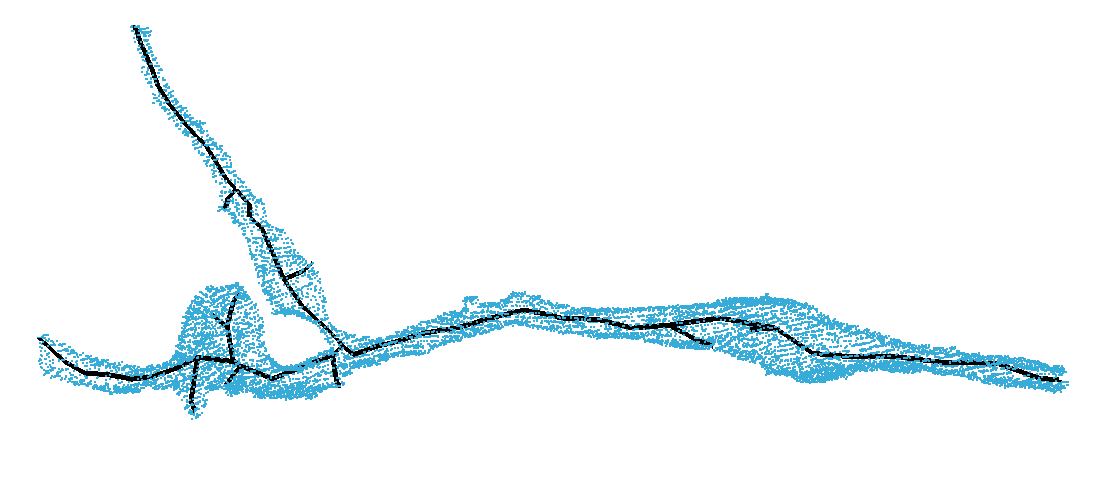
\includegraphics[width=0.8\linewidth]{./figures/split-proposal.png}
	\caption{An example where the input segmentation incorrectly merged two neurons together. The black circle indicates the junction from the skeletonized representation.}
	\label{fig:proposal}
\end{figure}

After locating these potentially erroneous segments, we will run a watershed algorithm on the affinities that forces the voxels into two segments.
This watershed algorithm will provide two seeds on opposite sides of the discovered junction.
The surface separating the two segments is our ``split'' candidate.
We will extract a cubic region of interest around this candidate and input the region into our previously discussed merge classifier.
If the classifier suggests that the segments belong to one neuron, we will ignore the split candidate.
Otherwise we will divide this segment based on the candidate.
With a synaptic classifier, we can further constrain the watershed algorithm to only propose splits where pre- or post-synaptic connections occur on one side.
This process will run recursively for a given segment in case more than two neurons are improperly merged.
